\section{Results}\label{sec:results}
\subsection{Simulation: validating the statistics (RQ1, RQ2, RQ4)}\label{sec:sim}
\paragraph{Interval coverage (RQ1).} Figure~\ref{fig:coverage} shows coverage of nominal 95\% intervals for the benchmark score ($\sigma_b=1.5$, interaction sd $0.5$). With one run per task the pooled binomial intervals are fine (they are exact in that case). With three runs they cover \covWilsonThreeRuns{} of the time and with ten runs only \covWilsonTenRuns{} (100 tasks), as the design effect predicts. A runs-only bootstrap is worse (\covRunsTenRuns). The task bootstrap, its BCa variant and the hierarchical beta-binomial interval stay close to nominal (task bootstrap: \covBootTenRuns{} at ten runs; BCa \covBCaTenRuns; beta-binomial \covBBTenRuns), and the two-stage bootstrap is conservative (\covTwoTenRuns). Coverage of the task bootstrap for pass$^k$ ranges between \covPassKMin{} and \covPassKMax{}. Full numbers are in Appendix~\ref{app:tables}.
\begin{figure}[t]
\centering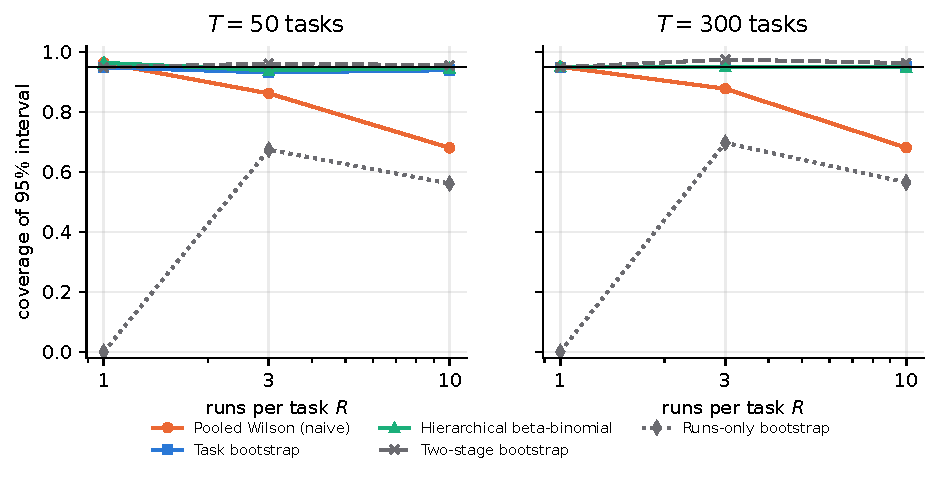
\includegraphics[width=\linewidth]{figures/coverage.pdf}
\caption{Coverage of nominal 95\% intervals for the benchmark score as runs per task grow (task sd $1.5$, interaction sd $0.5$, true score $\approx 0.43$). Pooling all runs breaks down already at three runs.}\label{fig:coverage}
\end{figure}

\paragraph{Robustness of coverage (E3).} The ranking of methods holds across prevalence and task heterogeneity, but the task bootstrap is not uniformly near nominal (Figure~\ref{fig:covrob}). For $T\ge50$ and $R>1$ it covers \covrobBootMin{}--\covrobBootMax{} and the beta-binomial interval \covrobBBMin{}--\covrobBBMax{}. With $T=20$, one run per task and extreme prevalence with homogeneous tasks the percentile bootstrap covers only \covrobBootSmallMin{}--\covrobBootSmallMax{} (BCa: from \covrobBCaSmallMin{}) because the resampled score is nearly degenerate; the pooled Wilson interval is exact there and should be preferred. The runs-only bootstrap has zero coverage at $R=1$ (\covrobRunsOnlyOne{}) because it sees no variation. The pooled Wilson interval fails only when runs are clustered \emph{and} tasks differ: at ten runs and task sd $1.5$ it covers \covrobWilsonMin{}--\covrobWilsonMax{}, and it is roughly nominal when tasks are nearly homogeneous. Our recommendation is therefore conditional: task-level intervals when $R>1$ or $T\ge50$, and an exact binomial interval for very small single-run evaluations.
\begin{figure}[t]
\centering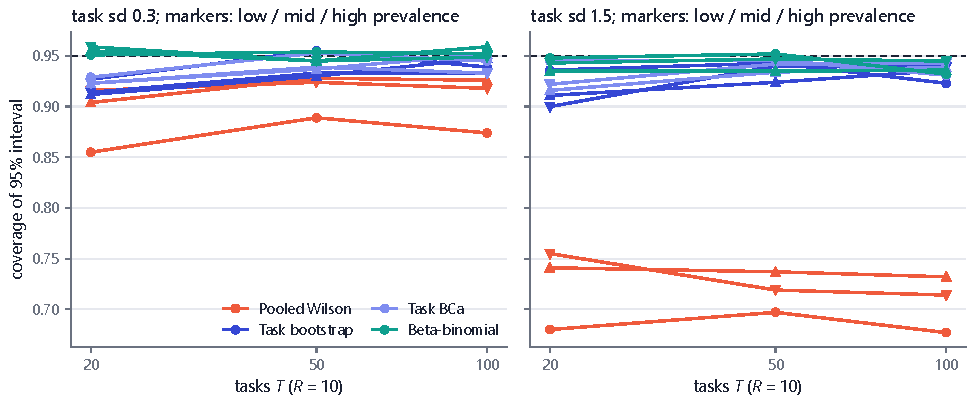
\includegraphics[width=\linewidth]{figures/coverage_robustness.pdf}
\caption{Coverage at ten runs per task for two task-heterogeneity levels and three prevalences (marker shape). Pooled Wilson loses coverage when tasks differ; the task-level methods approach the nominal level as $T$ grows.}\label{fig:covrob}
\end{figure}

\paragraph{Error rates of paired tests (RQ1).} With agent-by-task interaction sd $=1$, $T=100$ and ten runs per task, tests that treat each run as an independent pair reject a true null in \typeIPoolZ{} (two-proportion $z$-test) and \typeIPoolMc{} (run-level McNemar) of simulations, whereas the task-level sign-flip and bootstrap tests reject in \typeIPerm{} and \typeIBoot{} (Figure~\ref{fig:typeI}). With smaller interaction (sd $0.5$) run-level McNemar is still liberal (\typeIPoolMcLow). The pooled $z$-test is not always anti-conservative (it ignores pairing and is conservative at small $R$), so the harm of pooling is a loss of validity rather than a uniform inflation. Across all cells with a true null the sign-flip test rejects between \typeIPermMin{} and \typeIPermMax{}.
\begin{figure}[t]
\centering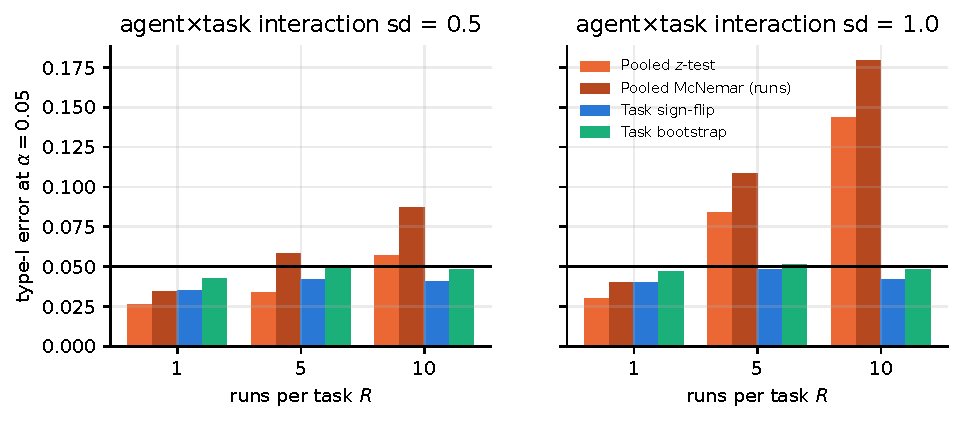
\includegraphics[width=\linewidth]{figures/typeI.pdf}
\caption{Type-I error at $\alpha=0.05$ for $T=100$ tasks and two agents of equal skill.}\label{fig:typeI}
\end{figure}

\paragraph{Weak null with skewed differences (E1).} The simulation above has symmetric per-task differences, where the sign-flip test is exact. We also generated paired differences with mean zero but heavy skewness (a rare large win offset by frequent small losses; skewness up to $5.5$). No procedure exceeded the pre-specified tolerance of 2 points over 5\% at $T\ge100$ (Figure~\ref{fig:asym}): across all cells the largest rejection rates were \asymMaxSF{} for the sign-flip test, \asymMaxSSF{} for its studentised version, \asymMaxBoot{} for the paired bootstrap and \asymMaxT{} for the paired $t$-test, with Monte Carlo error of about 0.6 points. The sign-flip tests are conservative on average (mean rejection \asymMeanSF{}); the bootstrap and $t$ tests are on average at nominal (\asymMeanBoot{}) but occasionally 1--2 points above it. We therefore keep the sign-flip test as the default, but we state its exactness only for symmetric differences.
\begin{figure}[t]
\centering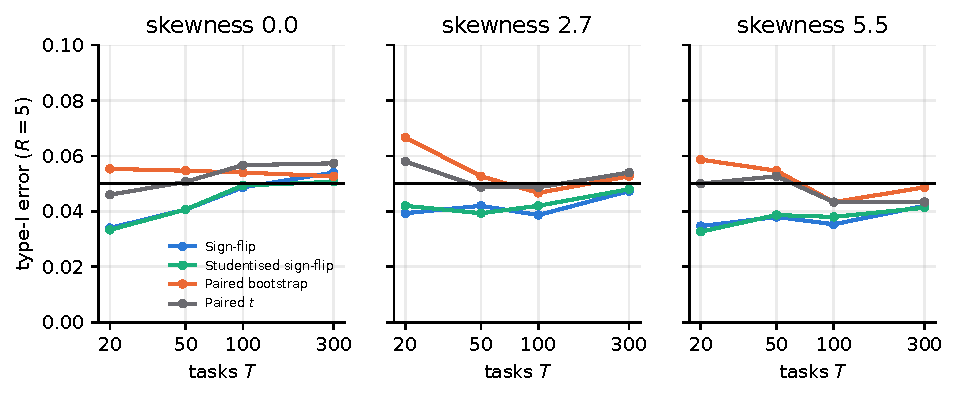
\includegraphics[width=\linewidth]{figures/asymmetric_null.pdf}
\caption{Type-I error at $\alpha=0.05$ with $R=5$ for paired differences with mean zero and increasing skewness (left to right).}\label{fig:asym}
\end{figure}

\paragraph{Tasks or repeats? (RQ2, E2).} In the original configuration (task sd $1.5$, interaction sd $0.6$) the standard error of the score difference at a fixed budget of \designBudget{} runs grows by a factor of \designSEratio{} between one and twenty runs per task, and power falls from \designPowerOne{} to \designPowerTen{} (ten runs) and \designPowerTwenty{} (twenty runs) (Figure~\ref{fig:design}); the analytic variance model predicts the simulated standard errors to within \designMaxSEgap{}. This is not a general law. Across nine configurations (E2, Figure~\ref{fig:alloc}) the standard-error ratio of ten versus one run per task is \allocRatioLow{} when the interaction sd is $0.2$ (repeats cost nothing) and \allocRatioHigh{} when it is $1.0$; the task standard deviation hardly matters, because the task main effect cancels in a paired difference. The cost-optimal number of runs per task for a task that costs ten runs is \allocRstarTenLow{} with small interaction and \allocRstarTenHigh{} with large interaction. If the pool of tasks is capped (for example at 120), the question changes and the extra budget must go to repeats. Analytic and simulated standard errors agree to within \allocMaxSEgap{} in E2. Repeats are not useless: they identify run noise and enable pass$^k$.
\begin{figure}[t]
\centering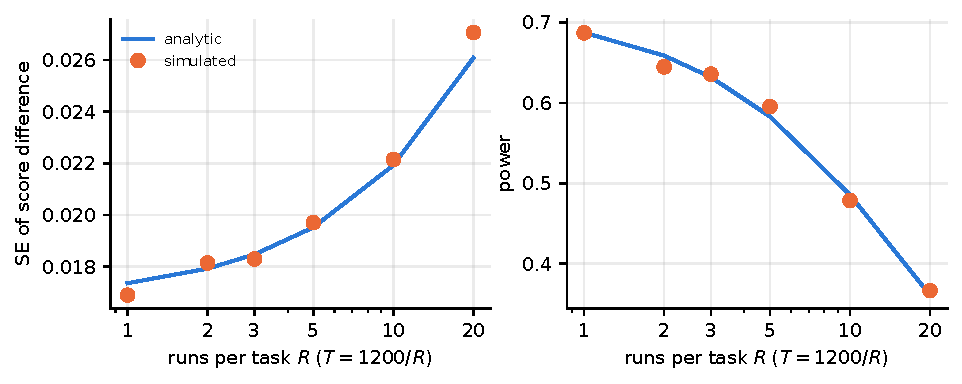
\includegraphics[width=\linewidth]{figures/design.pdf}
\caption{Fixed budget $B=1200$ runs, $T=B/R$ tasks. Left: standard error of the difference between two agents; right: power of the paired $t$-test.}\label{fig:design}
\end{figure}
\begin{figure}[t]
\centering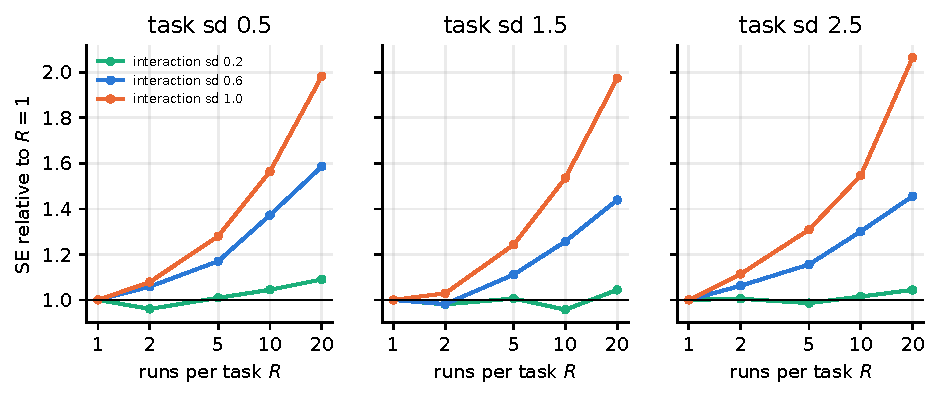
\includegraphics[width=\linewidth]{figures/allocation.pdf}
\caption{Standard error of the score difference at fixed budget relative to one run per task, for three task heterogeneities and three interaction levels. Curves are flat when the interaction is small.}\label{fig:alloc}
\end{figure}

\paragraph{Sequential evaluation (RQ4).} Applying a fixed-sample test after every task (``peeking'') and stopping at the first $p<0.05$ gives \seqNullPeek{} false positives under the null, against \seqNullSeq{} for the confidence sequence and \seqNullFixed{} for the fixed-$n$ test (Figure~\ref{fig:seq}). The price is power: with a true difference of \seqMidDiff{} points the sequence decides in \seqPowerSeqMid{} of runs against \seqPowerFixedMid{} for the fixed-$n$ test at the full budget of \seqBudget{} tasks. When the effect is large it stops early (median \seqLargeMedianTasks{} tasks for the largest difference). Confidence sequences buy the right to stop at any time; they do not make evaluation cheaper at a given power.
\begin{figure}[t]
\centering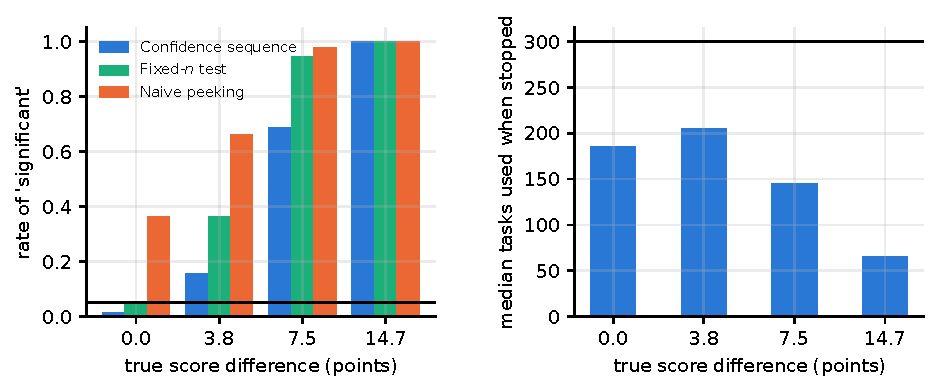
\includegraphics[width=\linewidth]{figures/sequential.pdf}
\caption{Sequential comparison, $R=3$ runs per task. Left: fraction declared significant (the line marks 5\%). Right: median number of tasks used when the sequence stops.}\label{fig:seq}
\end{figure}
Equivalence is only possible with a margin (E5, \seqmReps{} replications per cell). With margin zero ``equivalent'' was never declared (\seqmZeroMarginEquiv) and, for two agents of identical skill, the sequence stayed undecided in \seqmUndecidedTie{} of runs within 300 tasks: absence of a decision is not equivalence. With a margin of 10 points and a true gap of zero, equivalence was declared in \seqmEquivTrueTie{} of runs (median \seqmEquivTrueTieTasks{} tasks). When the true gap exceeded the margin, equivalence was declared in at most \seqmFalseEquivMax{} of runs, below $\alpha$, as the theory requires. Narrow margins are rarely reachable with 300 tasks.

\paragraph{Ranking uncertainty and near ties (RQ3, E6).} Bootstrap rank intervals are conservative for the population ranking (coverage \rankCovMin--\rankCovMax{} for nominal 95\%), and $P(\mathrm{best})$ is reasonably calibrated, noisily at $T=50$ (Figure~\ref{fig:rankcal}). In a six-agent leaderboard with one exactly tied pair and one pair \rankpwCloseTrue{} points apart, Holm-adjusted tests rejected the tied pair in at most \rankpwFWE{} of replications in every cell (the family-wise error is controlled and the procedure is conservative), but separated the close pair in only \rankpwCloseRej{} of replications even with 500 tasks and three runs per task (and \rankpwCloseRejSmall{} with 50 tasks). Small gaps are, in practice, not resolved by realistic benchmark sizes.
\begin{figure}[t]
\centering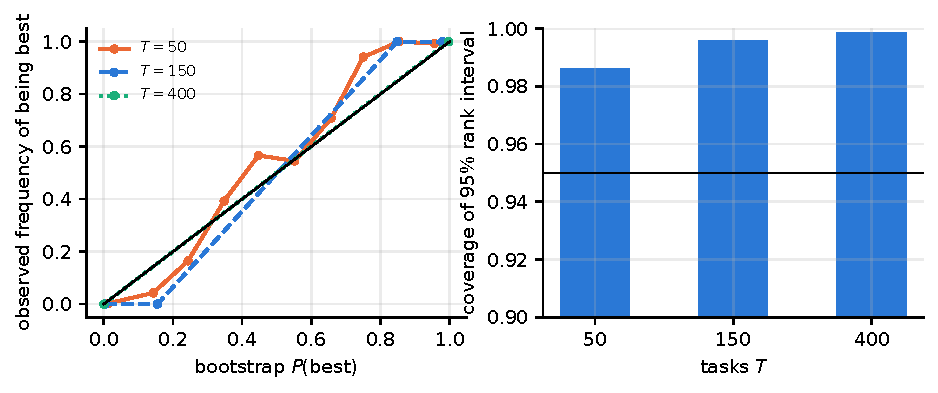
\includegraphics[width=\linewidth]{figures/ranking_calibration.pdf}
\caption{Six agents of known skill. Left: calibration of bootstrap $P(\mathrm{best})$. Right: coverage of the 95\% rank interval.}\label{fig:rankcal}
\end{figure}

\subsection{Re-analysis of public results (RQ3)}\label{sec:public}
\paragraph{SWE-bench Verified.} The \sweNAgents{} entries yield \sweNPairs{} agent pairs. After Holm adjustment \sweFracHolm{} are distinguishable at $\alpha=0.05$ (\sweFracBH{} with Benjamini--Hochberg; \sweFracRaw{} without correction), so \sweIndistHolm{} cannot be separated; ``cannot be separated'' means not detected, not equal. The result is driven by the score gap (Figure~\ref{fig:swe}): pairs 2--5 points apart are separable in \sweGapSmallHolm{} of cases after correction, pairs 5--10 points apart in \sweGapMidHolm{}, and larger gaps almost always. The smallest distinguishable gap is \sweMinGap{} points and the median is \sweMedGap. The top entry (\sweTopScore) has a 95\% rank interval of 1--\sweTopRankHi{} and probability \sweTopPBest{} of being best.
\begin{figure}[t]
\centering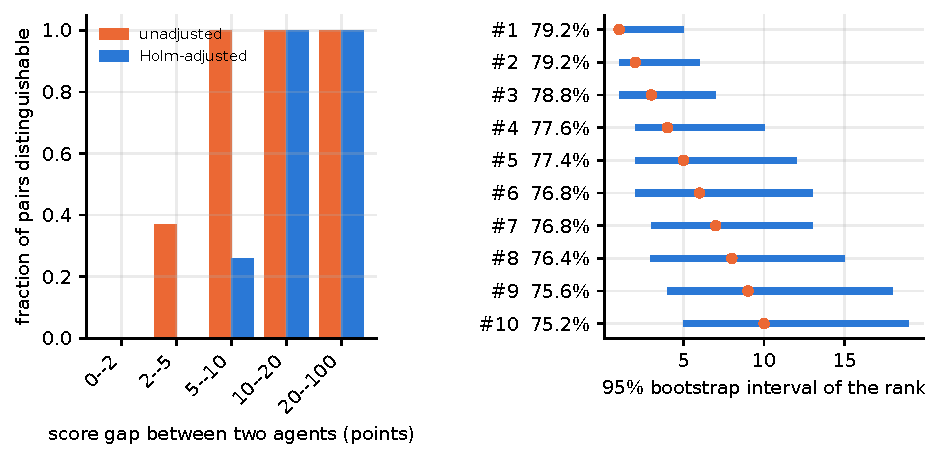
\includegraphics[width=\linewidth]{figures/swebench.pdf}
\caption{SWE-bench Verified, \sweNAgents{} public entries. Left: fraction of pairs distinguishable by score gap. Right: top-10 scores with 95\% bootstrap rank intervals.}\label{fig:swe}
\end{figure}

\paragraph{Sensitivity to undocumented evaluation details.} The headline count of adjacent positions depends on the entries retained (Table~\ref{tab:swerobust}). Among all entries, \sweAllAdjHolm{} of adjacent leaderboard positions are distinguishable after Holm over \emph{all} pairs (\sweAllAdjRaw{} without correction). Restricting to entries whose coverage of the 500 instances could be verified gives \sweCovAdjHolm{}; restricting to entries that declare a single attempt (\sweNSingle{} entries) gives \sweSingleAdjHolm{}, because with fewer, more spread-out entries adjacent gaps are larger. The share of separable pairs is stable (\sweCovFracHolm{} coverage-verified, \sweSingleFracHolm{} single-attempt, \sweBothFracHolm{} both). The qualitative conclusions, that most pairs but almost no adjacent positions are separable, therefore hold across the subsets, whereas the earlier claim that \emph{none} of the adjacent positions is distinguishable is not robust: it is true only for the full set. Many entries are best-of-$n$ or multi-sample systems and different scaffolds, budgets and dates are mixed; the comparison is of leaderboard rows, not of models.
\begin{table}[t]
\centering\small
\caption{SWE-bench Verified sensitivity analysis. ``Adjacent'' counts distinguishable neighbouring leaderboard positions; Holm is applied over all pairs of the subset.}\label{tab:swerobust}
\begin{tabular}{lrrrr}
\toprule
Subset & Entries & Pairs separable (\%) & Adjacent, Holm & Adjacent, unadjusted \\
\midrule
All entries & 129 & 71.7 & 0/128 & 2/128 \\
Coverage verified & 110 & 71.7 & 1/109 & 3/109 \\
One attempt declared & 41 & 69.3 & 3/40 & 6/40 \\
Both & 37 & 68.5 & 2/36 & 5/36 \\
\bottomrule
\end{tabular}

\end{table}

\paragraph{$\tau$-bench.} For gpt-4o versus Claude 3.5 Sonnet with four trials per task, the retail gap is \tauRetailDiff{} points (95\% task-bootstrap interval \tauRetailCI), task-level sign-flip $p=\tauRetailPPerm$ ($p=\tauRetailPHolm$ after Holm adjustment over the two domains); the pooled-runs $z$-test gives $p=\tauRetailPPool$. The task-level exact McNemar test on per-task majority outcomes, which discards run-level information, gives $p=\tauRetailPTaskMc$, so the retail result is not independent of the choice of test. In airline the gap is \tauAirlineDiff{} points \tauAirlineCI{} with $p=\tauAirlinePPerm$ (pooled $p=\tauAirlinePPool$): not detected with \tauAirlineTasks{} tasks, which does not show that the two models are equal. Plug-in power calculations suggest about \tauAirlineNeed{} tasks would be needed at the observed airline gap (retail: \tauRetailNeed{}), but these figures are very uncertain: a task bootstrap of the pilot gives 95\% intervals of \tauAirlineNeedLo{}--\tauAirlineNeedHi{} (airline) and \tauRetailNeedLo{}--\tauRetailNeedHi{} (retail) tasks. Variance is dominated by run noise (\tauAirlineRunShare{} airline, \tauRetailRunShare{} retail) and task difficulty (\tauAirlineTaskShare, \tauRetailTaskShare), with agent-by-task interaction of \tauAirlineInterShare{} and \tauRetailInterShare. Figure~\ref{fig:tau} contrasts pass@$k$ with pass$^k$: both models look strong when one success in $k$ suffices and much weaker when all $k$ must succeed. The data cover two models and two domains, and the model versions are those of the released trajectories.
\begin{figure}[t]
\centering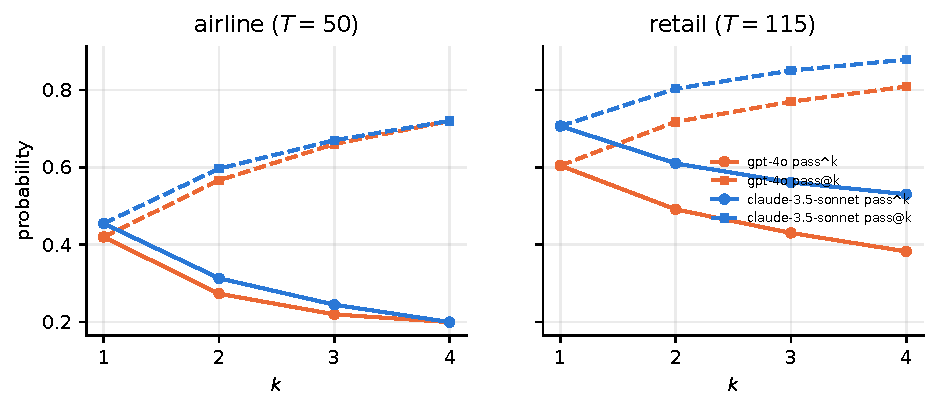
\includegraphics[width=\linewidth]{figures/taubench.pdf}
\caption{$\tau$-bench, four trials per task: pass$^k$ (solid) falls and pass@$k$ (dashed) rises with $k$.}\label{fig:tau}
\end{figure}

\IfFileExists{sections/real.tex}{\subsection{Local open-weight models (RQ5)}\label{sec:real}
\paragraph{Setup and headline numbers.} \realNModels{} models, \realNTasks{} tasks, \realNRuns{} runs each (\realNAttempts{} runs in total). Success rates range from \realWorstScore{} (\realWorstModel) to \realBestScore{} (\realBestModel); the full table with pass$^k$ and per-family scores is in Appendix~\ref{app:real}. Figure~\ref{fig:real} (left) shows 95\% task-bootstrap intervals. Scores here combine two things: protocol validity (does the model emit a parseable action in the uniform text protocol?) and task competence. The quantised variant \texttt{qwen2.5-3b-q2} never produced a parseable action (\realFloorNoAction{} of its runs end with no tool call), so its score of zero measures protocol failure and says nothing about the underlying agent; we keep it as a degenerate control rather than dropping it silently, and it contributes to the variance decomposition and the pair counts as a floor. Without it, \realNIndistNoQtwo{} of the \realNPairsNoQtwo{} remaining pairs are not separable after Holm (recomputed from the stored pairwise $p$-values); the variance decomposition and the rankings without it could not be recomputed because the per-run outcomes are not stored (Appendix~\ref{app:repro}). Backend errors (\realBackendErr{} runs, \realBackendErrShare{}) are scored as failures. Results are specific to this protocol and these quantised models.
\begin{figure}[t]
\centering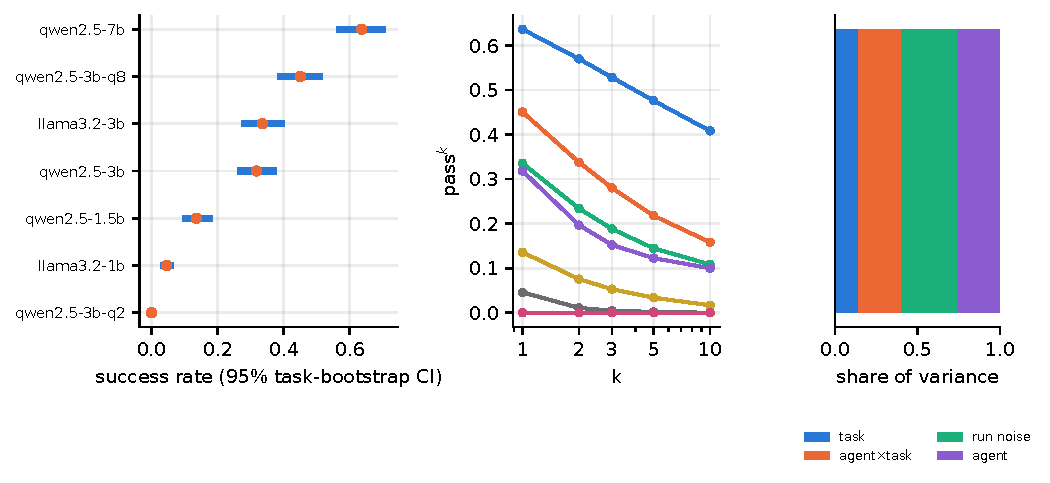
\includegraphics[width=\linewidth]{figures/real_main.pdf}
\caption{Local models on the \realNTasks-task core suite, \realNRuns{} runs per task. Left: success rate with 95\% task-bootstrap interval. Middle: pass$^k$. Right: variance decomposition of the full agents-by-tasks-by-runs array.}\label{fig:real}
\end{figure}

\paragraph{Reliability is much lower than the headline score.} The best model's score of \realBestScore{} falls to \realBestPassThree{} for pass$^3$ and \realBestPassTen{} for pass$^{10}$: a model that solves a task on average does not solve it every time. Run noise accounts for \realRunShare{} of the variance of single runs, task difficulty for \realTaskShare, agent-by-task interaction for \realInterShare{} and agent identity for \realModelShare. The agent share describes the spread of these seven fixed models, not a population variance. Run noise is of the same order as the quantity of interest, so a one-run evaluation is a noisy measurement even here.

\paragraph{Ranking: the hypothesis is only partly borne out.} Because the models differ a lot in capability, the ranking is well determined: \realNIndist{} of \realNPairs{} pairs are not separable after Holm correction (\realClosestA{} versus \realClosestB{}, a gap of \realClosestDiff{} points, adjusted $p=\realClosestP$), and the split-half rank correlation is \realSplitTau. This contrasts with SWE-bench, where scores are close; the statistical problems are most severe when systems are close, not absent otherwise. A plug-in power calculation says that resolving a 5-point difference between two of these agents at 80\% power needs about \realTasksNeeded{} tasks at ten runs per task, more than three times the suite size, and the minimum detectable difference of the current design is \realMDE{} points; both are estimates from one pilot and carry the uncertainty documented for $\tau$-bench above. With the cost model of Section~\ref{sec:power}, the optimal number of runs per task is \realOptRuns{} when a task costs as much as ten runs.

\subsection{Ablations on real data}\label{sec:ablation}
\paragraph{Tasks versus runs.} The sub-designs are random subsets of the same \realNTasks{} tasks and ten runs, compared with the ranking and the significant pairs of the full data. The full-data ranking shares observations with every subsample and is itself an estimate, so this measures \emph{internal stability relative to the full observed sample}, not recovery of an independently known population ranking; the pairs that are significant in the full data are also selected by the same data, so sign agreement among them is optimistic. Recovery of a known ranking is examined in the simulation (E6, Figure~\ref{fig:rankcal}); a split-sample analysis on independent halves would require the per-run outcomes, which are not stored. Sub-sampling the real data (Figure~\ref{fig:realabl}), a ranking from all \realNTasks{} tasks with one run per task has Kendall $\tau=\ablTauOneRun$ with the full-data ranking and separates \ablFracOneRun{} of the pairs, against \ablFracAllRuns{} with ten runs. With only \ablFewTasks{} tasks and one run the ranking correlation is $\tau=\ablTauFewTasks$ and only \ablFracFewTasks{} of pairs are separated. Since the large gaps are easy, rank correlation saturates quickly; the number of \emph{separated pairs} is the informative measure and it keeps growing with both tasks and runs. We did not repeat the fixed-budget comparison of Section~\ref{sec:sim} on real data, so the simulation result on tasks versus runs is neither confirmed nor refuted here.
\begin{figure}[t]
\centering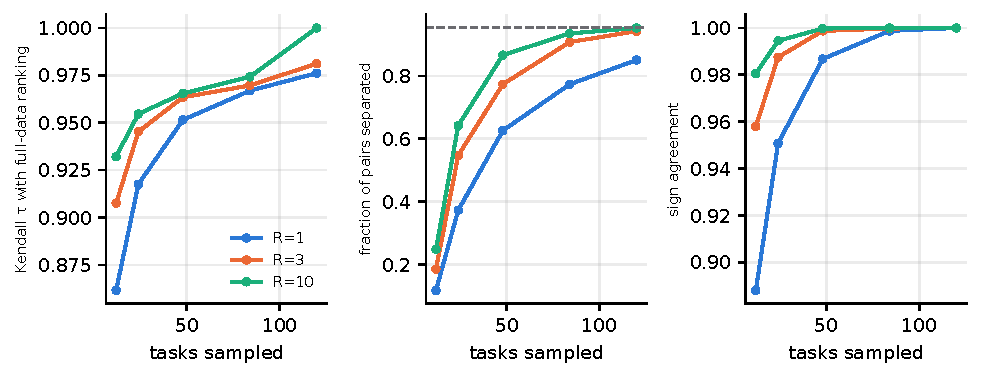
\includegraphics[width=\linewidth]{figures/real_ablation.pdf}
\caption{Sub-designs of the real data (random subsets of tasks and runs, 200 draws). Left: Kendall $\tau$ with the full-data ranking. Middle: fraction of the \realNPairs{} pairs separated (paired $t$-test, Holm); the dashed line is the full data. Right: sign agreement for pairs that are significant in the full data. The reference is the full-data result, which shares observations with every subsample, so all panels measure stability relative to the observed sample, not accuracy against a known truth.}\label{fig:realabl}
\end{figure}

\paragraph{Sequential stopping.} Applying the confidence sequence to tasks in random order, \seqRealDecided{} of the \seqRealNSig{} pairs that are significant on the full data are decided before the tasks run out, with a median of \seqRealMedTasks{} tasks. This re-orders existing results; it is not a live stopping experiment. Large gaps are settled after a few tens of tasks; close pairs are not decided within the suite, as in the simulation.

\paragraph{Cost profile.} Figure~\ref{fig:realprof} reports tokens and wall-clock per run. The weakest functioning model, \realMaxStepLimitModel, hits the step limit in \realMaxStepLimit{} of runs and consumes the most tokens: failure is not cheap, so cost per success varies more than cost per run. Wall-clock was measured with four parallel workers on one machine and is indicative only.
\begin{figure}[t]
\centering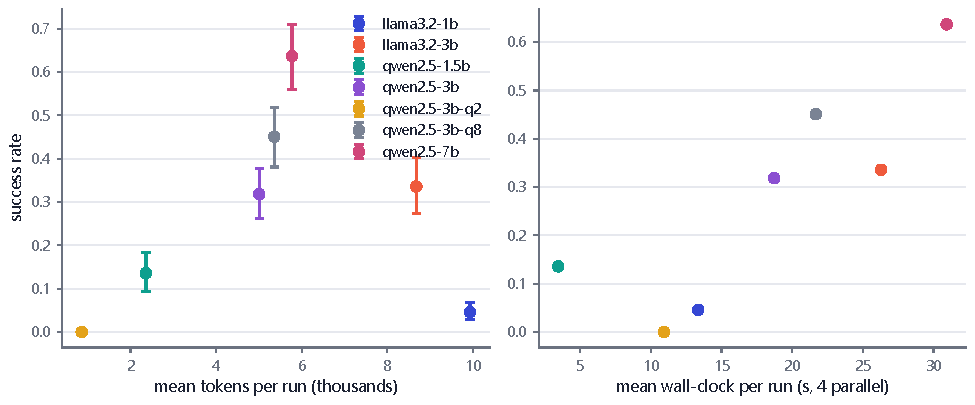
\includegraphics[width=\linewidth]{figures/real_profile.pdf}
\caption{Success rate against mean tokens (left) and wall-clock (right) per run.}\label{fig:realprof}
\end{figure}
}{}
